\section{Theorie}
\label{sec:Theorie}

\subsection{Eigenschaften von Linsen}
Linsen bestehen meistens aus optisch dichteren Material als die Luft die sie
umgeben. Es wird zwischen Sammellinse und Zerstreuungslinse unterschieden. Die
Sammellinse bündelt paralleles Licht in einem Brennpunkt. Sowohl Bildweite $b$ als auch
Brennweite $f$ sind positiv und das entstehende Bild kann auf einen Schirm sichtbar gemacht werden.
Für eine Zerstreuungslinse ist die Bildweite und die Brennweite negativ. In Abbildung 1 sind diese
beiden Linsen dargestellt.

\begin{figure}[H]
  \centering
  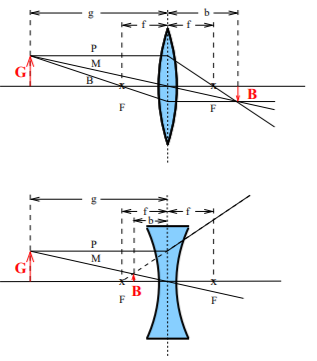
\includegraphics[height=5cm]{linsen.PNG}
  \caption{Strahlengang einer Sammellinse und einer Zerstreuungslinse \cite{sample}.}
  \label{fig:biegungbild1}
\end{figure}

Aus der Bildkonstruktion und den Strahlensätzen lässt sich das Abbildungsgesetz herleiten.
\begin{align}
  V =\frac{B}{G} = \frac{b}{g}
\end{align}

Dabei ist $V$ der Abbildungsmaßstab, $B$ die Bildgröße, $G$ die Gegenstandsgröße und $g$ die Gegenstandsweite, welche
auch in Abbildung 1 dargestellt sind.
Für dünne Linsen, wie in der Abbildung, folgt daraus die Linsengleichung:
\begin{align}
  \frac{1}{f} = \frac{1}{b} + \frac{1}{g}
\end{align}

Für dicke Linsen, wie in Abbildung 2 dargestellt, wird die Mittelebene durch zwei Hauptebenen $H$ und $H'$ ersetzt
an denen die Strahlen gebrochen werden.

\begin{figure}[H]
  \centering
  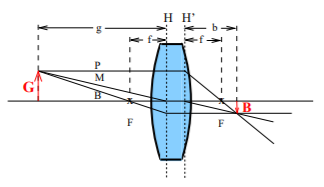
\includegraphics[height=5cm]{dickelinse.PNG}
  \caption{Strahlengang einer dicken Sammellinse \cite{sample}.}
  \label{fig:biegungbild1}
\end{figure}

Die einzelnen Größen werden zur jeweiligen Hauptebene bestimmt, wodurch die Linsengleichung
gültig bleibt.

Achsenfernere Strahlen werden stärker gebrochen, wodurch Abbildungsfehler entstehen. Werden diese
ausgeblendet entsteht wieder ein scharfes Bild.

\subsection{Bestimmung der Brennweite mit der Methode von Bessel}
Der Abstand zwischen Gegenstand und Bild bleibt fest. Die Position der Linse wird variiert,
sodass zwei Orte für die Linse gefunden werden, wo das Bild scharf ist. Für diese
Stellungen können Bildweite und Gegenstandsweite vertauscht werden.
\begin{align*}
  b_1 = g_2 \\
  b_2 = g_1
\end{align*}
Daraus lässt sich für die Brennweite  die Gleichung 3 herleiten.
\begin{align}
  f = \frac{e^2 - d^2}{4e}
\end{align}

Hierbei ist $e$ der Abstand zwischen Gegenstand und Bild und $d$ der Abstand zwischen den
beiden Linsenpositionen. Diese sind in Abbildung 3 dargestellt.

\begin{figure}[H]
  \centering
  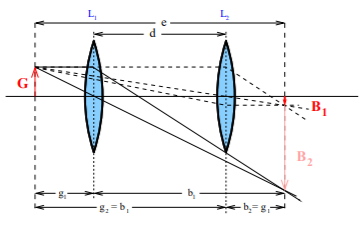
\includegraphics[height=5cm]{bessel.PNG}
  \caption{Geometrische Beziehungen für die Methode von Bessel \cite{sample}.}
  \label{fig:biegungbild1}
\end{figure}

\subsection{Bestimmung der Brennweite mit der Methode von Abbe}
Mit der Methode von Abbe wird die Brennweite eines Linsensystems mithilfe des Abbildungsmaßstabes bestimmt.
Aus Abbildung 4 lässt sich eine Formel für die Brennweite herleiten, hierfür müssen die Lagen
der Hauptebenen bekannt sein.

\begin{align}
  g'= g + h = f \cdot \left(1 + \frac{1}{V} \right) + h \\
  b' = b + h' = f \cdot (1+V) + h'
\end{align}

\begin{figure}[H]
  \centering
  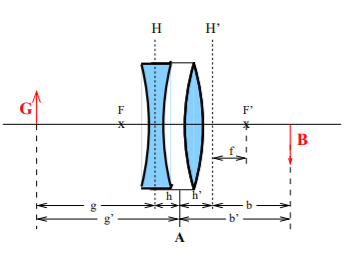
\includegraphics[height=5cm]{abbe.PNG}
  \caption{Geometrische Beziehungen eines Linsensystems \cite{sample}.}
  \label{fig:biegungbild1}
\end{figure}
